%----------------------------------------------------------------------------
%bb defines the bounding box for the pdf
%viewport defines the area of the pdf used
%in sidewaysfigure the last entry in bb moves the caption toward/away the pic
%in sidewaysfigure the second entry in bb moves the pic toward/away the caption
%----------------------------------------------------------------------------
\begin{figure}
\scalebox{0.7}[0.7]{
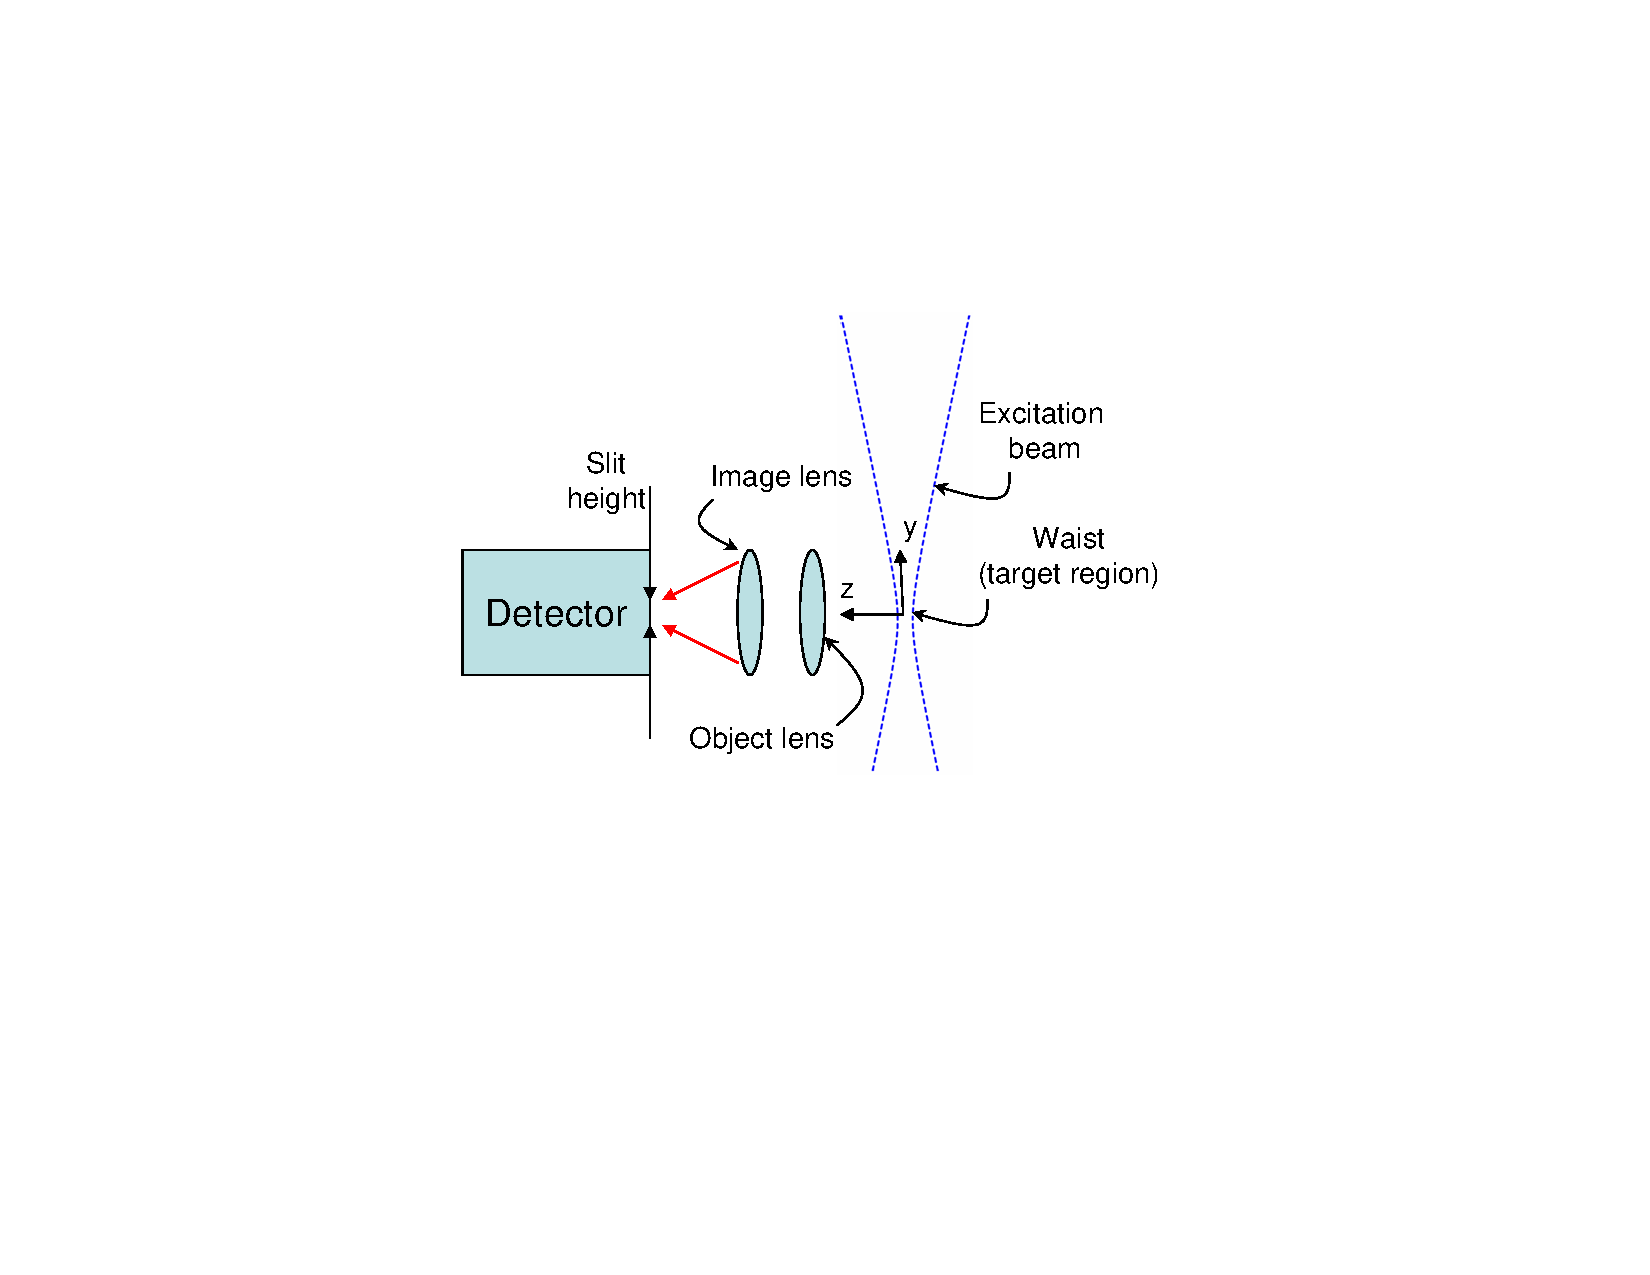
\includegraphics[bb=80 230 489 450]
{side_view_figure/side_view_figure.pdf}
}
\caption[Side view geometry]{Side view geometry. For the calculation in Figure \ref{side_view}, each object (image) lens is placed one focal length from the target region (detector input). The slit such that its long dimension (height) is oriented in the y--direction and its narrow dimension is oriented in the x--direction.}
\label{side_view_figure}
\end{figure}
%----------------------------------------------------------------------------
